\documentclass[lettersize, apacite, twoside, HRI]{apa_HRI}
\usepackage{times} % Required package for HRI journal format

% UTF8 support
\usepackage[utf8x]{inputenc}
\usepackage[T1]{fontenc}

\usepackage{graphicx}
\graphicspath{{figs/}}
\usepackage{tikz}
\usetikzlibrary{shapes}
%
\usepackage{amsmath} 
\usepackage{mathptmx}      % use Times fonts if available on your TeX system
%
\usepackage{color, soul}
\usepackage{url}
\usepackage[numbers, square, comma, sort&compress]{natbib}
\usepackage{multirow}
\usepackage{array}
\usepackage{fixltx2e}
\usepackage{textcomp}

\usepackage[draft, nomargin, marginclue, footnote]{fixme}
\fxsetup{targetlayout=color}

\rightheader{Journal of Human-Robot Interaction}
\leftheader{Fink et al.}

\newcommand{\eg}{{\textit{e.g.~}}}
\newcommand{\etal}{{\textit{et al.~}}}
\newcommand{\ie}{{\textit{i.e.~}}}

\hyphenation{com-mon-ly}


\title{On the Dynamics of Anthropomorphism in Robotics
}

\author{Julia Fink, Séverin Lemaignan, Pierre Dillenbourg}
\affiliation{ Computer-Human Interaction in Learning and Instruction (CHILI) \\
              Ecole Polytechnique Fédérale de Lausanne (EPFL) \\
              CH-1015 Lausanne, Switzerland
}

\abstract{While anthropomorphism in robotics is a commonly discussed trait of
HRI, it is paradoxically an overlooked research topic. This article
attempts first at providing a comprehensive synthesis of the social
phenomenon of \textit{perceiving human-like characteristics in non-human
agents and attributing those characteristics to robots}. We draw on
social sciences and psychology, as well as on a critical survey of
existing literature in the HRI community, to ground the concept of
\textit{anthropomorphism}. We further briefly present different kinds
of \textit{anthropomorphic design} of robots and outline their role in
social robotics\fxfatal{do we really do?}. We then suggest to go beyond the traditional
perception of anthropomorphism as a static feature of a system: we propose to
understand anthropomorphism as a dynamic, non-monotonic and
context-dependent process, which evolves over time and accounts for
special events like the so-called \textit{novelty effect}. To this end,
we introduce a model of anthropomorphism that analyzes the phenomenon
along three interaction phases. These findings are supported by a long-term
study conducted in a real human environment.}



\keywords{Anthropomorphism, Design, Human-Robot Interaction, Social Issues in Robotics, Acceptance of Robots}

\begin{document}
\maketitle


%%%%%%%%%%%%%%%%%%%%%%%%%%%%%%%%%%%%%%%%%%%%%%%%%%%%%%%%%%%%%%%%%%%%%%%%%
%
%
%
%				INTRODUCTION
%
%
%
%%%%%%%%%%%%%%%%%%%%%%%%%%%%%%%%%%%%%%%%%%%%%%%%%%%%%%%%%%%%%%%%%%%%%%%%%


\section{Anthropomorphism}
\label{sec:intro}

%DEFINITION OF ANTHROPOMORPHISM

The essence of anthropomorphism is perceiving human-like characteristics in either real or imagined non-human agents. According to Epley \textit{et al.} \cite{epley_when_2008}, these human-like characteristics may include physical appearance (such as a religious agent believed to look human-like), emotional states perceived to be uniquely human, or inner mental states and motivations. Real or imagined non-human agents can be "anything that acts--or is believed to act--with apparent independence, including non-human animals, natural forces, religious agents, technological gadgets, or mechanical devices". Such anthropomorphic representations are important determinants of how a person behaves towards these agents, or how a person may behave \fxnote*{in light?}{in light} of these agents.

%ANTHROPOMORPHISM AS SUBJECT IN HCI AND HRI	
	
In this context, anthropomorphism has received \fxnote*{contradict with intro}{remarkable attention} in the study of humans interacting with artificial entities, and has been a subject in Human-Computer Interaction (HCI) and Human-Robot Interaction (HRI). Following the \textit{Media Equation}, it has been described that people mindlessly react socially to computers \cite{reeves_media_1996}. The phenomenon has also been observed with virtual characters \hl{cite [50, 100] in rosenthal-von der P{\"u}tten (2013)}, and more recent studies investigated how far people ascribe personality or intentions to artificial agents \hl{references}\fxnote{Rosenthal is not enough?} and whether they show empathetic behavior toward robots \cite{rosenthal-vonderputten_experimental_2013}. The common base for this research is the assumption that humans perceive or react to a non-human agent or artifact as somewhat similar to a human.

We furthermore use in this article \emph{anthropomorphic effects} to denote the
observable correlates of anthropomorphism. These include, amongst others,
verbal behaviors (like the use of pronouns ``he/she''), kinesics (like hugging
the robot) or anticipation of certain robot's actions.

%CONTROVERSAL UNDERSTANDINGS OF ANTHROPOMORPHISM

However, not everything colloquially labeled as \emph{anthropomorphism} really is anthropomorphism. Different, even partially conflicting, understandings of anthropomorphism exist across and within disciplines \cite{duffy_anthropomorphism_2002}. Epley \textit{et al.} \cite{epley_when_2008} try to narrow down and clarify the understanding of anthropomorphism in psychology by explaining what it is \textit{not}. The authors list four things that anthropomorphism does not include: First, anthropomorphism does not include behavioral descriptions of observable actions. Anthropomorphism requires going beyond what is directly observable. Second, anthropomorphism does not merely entail animism, as animate life is not a uniquely human-like characteristic. Third, anthropomorphism does not include any requirement of reasoned or reflective endorsement of an inference (\hl{the strength of anthropomorphic inferences can vary} \footnote{for further explanation the reader may refer the original work \cite{epley_when_2008}.}).	Finally, anthropomorphism is not necessarily inaccurate. A psychological theory should take this (in)accuracy in anthropomorphism into account and predict variability in the tendency to perceive human-like traits in non-human agents\fxfatal{End of paragraph is unclear. We need to reformulate}.
	 

%ANTHROPOMOPRHIC DESIGN

Anthropomorphism represents just one of many examples of induction whereby "people reason about an unknown stimulus based on a better-known representation of a related stimulus" \cite{epley_when_2008}, in this case reasoning about a non-human agent based on representation of the self or humans. This supports the usual role we assign to anthropomorphism in robotics: the anthropomorphic design of a robot encourages people to reason about this unfamiliar system \emph{as if} it was a human. To increase this tendency, robots are designed with anthropomorphic forms (human-like forms or lifelike forms, in the broader sense), or are able to display and use human-social behavior.
	
	

\paragraph{Anthropomorphism in robotics} Literature on anthropomorphism in robotics is quite diverse and one strives hard to extract a coherent conclusion. There is no commonly accepted definition about the terms used and the terminology is not clear. However the terms \textit{anthropomorphic or human-like are often used as if their meanings are clear and agreed upon"} \cite{persson_anthropomorphism_2000}. Consequently, Duffy \cite{duffy_anthropomorphism_2002} argues that terms might even be misused. For instance, some researchers refer to \textit{"the robot's level of anthropomorphism"} \cite{bartneck_is_2007}, however, others argue that anthropomorphism emerges in the \textit{interaction} between the technology and the user, thus a system or an artifact does not "contain anthropomorphism" \textit{per se} \cite{persson_anthropomorphism_2000} but only gives rise to the process of anthropomorphizing in a given user and situation. Further, robotics is a multi-disciplinary field and researchers from very different domains might have diverse or even contradictory understandings of anthropomorphism. Epley \textit{et al.} \cite{epley_seeing_2007} notice that despite the fact that anthropomorphism in the perception of non-human agents is commonly observed, it is poorly understood. The phenomenon itself has been found to be very complex but sometimes subtle and hard to study. Another constraint that limits the reliability of some findings is, that most experiments on anthropomorphism are conducted in controlled lab-settings during short-term interactions. This experimental setting (short term and laboratory context) can be critical when studying a social phenomenon like anthropomorphism and possibly lead to over-interpretations. Some studies also seem to contrast two or more different anthropomorphic and mechanical systems that might not be appropriate for comparison under the given context and research question. \hl{say more}

To sum it up, while anthropomorphism in robotics is a commonly discussed and studied trait of human-robot interaction, we think it is paradoxically an overlooked research topic. The understanding of anthropomorphism in robotics seems to not take into account the wide range of phenomena that it encompasses. The traditional understanding of anthropomorphism in robotics to date considers two main factors that account for the social phenomenon: the characteristics of \textbf{1) the robot's design} (degree of human-likeness) and the psychological determinants in \textbf{2) the human user} (see \cite{epley_seeing_2007}). It has been shown that both these factors can facilitate or hinder anthropomorphism. We propose to go beyond this traditional perception of anthropomorphism as a static feature of HRI: Based on Persson \textit{et al.}'s~\cite{persson_anthropomorphism_2000} argumentation that anthropomorphism is a multi-layered phenomenon which arises in different levels, we suggest to understand anthropomorphism as a \emph{dynamic}, \emph{context-dependent} process. To this end, we apply Persson \textit{et al.}'s six levels on anthropomorphism to HRI and introduce three \emph{interaction phases}. These interaction phases of anthropomorphism reflect also the results of a long-term study that we conducted in a real human environment and provide an account of the so-called \textit{novelty effect}. We also draw attention to two new determinants of anthropomorphism, namely, the context of use and the fact of getting used to a system over time. We propose to add these two aspects as a third factor, the characteristics of \textbf{3) the interaction} (time and space), to the previous two factors of anthropomorphism (robot and user). 


%% -> Commented out the overview as it does not match what we actually present... maybe we need a new one?
% We would further like to review and discuss research on anthropomorphism in robotics and human-like design of robots. We first provide a comprehensive understanding of the phenomenon drawing on theories from developmental psychology and cognitive sciences. We then present the trends of different kinds of anthropomorphic forms in robots and discuss their role in social robotics. The article integrates related work from human-robot interaction studies, reporting on findings from experiments with human subjects interacting with and evaluating various types of systems. We try to give a coherent view on the topic, outline similarities and antithetic findings, and contribute to a better understanding of anthropomorphism in robotics, and the acceptance of human-like characteristics in robots. We also aim to constructively discuss anthropomorphic design of personal and socially interactive robots. 
	

%%%%%%%%%%%%%%%%%%%%%%%%%%%%%%%%%%%%%%%%%%%%%%%%%%%%%%%%%%%%%%%%%%%%%%%%%
%
%
%
%				ANTHROPOMORPHISM: EXPLANATIONS & BACKGROUND
%
%
%
%%%%%%%%%%%%%%%%%%%%%%%%%%%%%%%%%%%%%%%%%%%%%%%%%%%%%%%%%%%%%%%%%%%%%%%%%



\section{Anthropomorphism as a Social Phenomenon}
\label{sec:origins-anthropomorphism}

The term \textbf{anthropomorphism} is used in different senses throughout natural sciences, psychology, Human-Computer Interaction, and Human-Robot Interaction \cite{duffy_anthropomorphism_2003}. Originally, anthropomorphism comes from the Greek \textit{`anthropos'} for `man' (or `human') and \textit{`morphe'} for `form/structure' (or `shape'). It can be understood as people's tendency to think of objects as if they had human characteristics, and consequently, attribute / ascribe specific human characteristics to these non-human entities and artifacts (including animals, and robots) \cite{duffy_anthropomorphism_2003,schmitz_concepts_2011}. Apart from anthropomorphism there is also \textbf{animism}, the \textit{"attribution of life to the nonliving"} \hl{in Schmitz 2011, cite Piaget original text!}. Often synonymously used to animism is \textbf{zoomorphism}, which describes the case when non-lifelike objects are associated with animalistic attributes, excluding human-specific traits. Both anthropomorphism and zoomorphism can be embraced by the concept of \textbf{life-likeness}. \footnote{The inverse process would be called dehumanization \cite{haslam_dehumanization:_2006}, or mechanomorphism \cite{caporael_anthropomorphism_1986}.}
		
Commonly, anthropomorphism can also be understood as \textbf{humanization} or \textbf{personification} of anything other than a human being. The phenomenon of personifying something has ancient roots, \textit{e.g.} in mythology but also in storytelling. In prehistoric artworks and illustrations, zoomorphic (animal-shaped) or anthropomorphic shapes were already used to represent natural forces or great spirits, for instance. A more recent example is Milo Winter's illustration from 1919, \textit{"The North Wind and the Sun"} (Figure \ref{fig:1}), in which both north wind and sun are given a human face (anthropomorphized). Similarly, when parents explain their children about nature, they tend to use anthropomorphisms, \textit{e.g.} saying the skies would cry when it rains. More generally, an explanation for why people anthropomorphize is that by doing so, the subject is made \emph{graspable}, \emph{understandable}, \emph{predictable}, and one feel \emph{more empathetic} toward it\fxnote{important part. Emphasize this 4 facets, eg by saying we build on top of them}. For instance, people commonly anthropomorphize their pets, ascribing mental states, intentions or feelings to them \cite{eddy_attribution_1993}. Interestingly, pet-ownership seems to have a significant impact on human-robot interaction: several studies suggest that pet-owners are more likely to anthropomorphize technologies and robots than non pet-owners \hl{references!}.

 \begin{figure}\centering
% Use the relevant command to insert your figure file.
% For example, with the graphicx package use
  
\includegraphics[scale=0.91]{north-wind.jpg}
  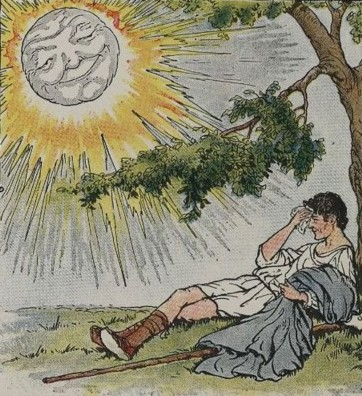
\includegraphics[scale=0.91]{sun.jpg}
% figure caption is below the figure
 \caption{Milo Winter illustration of Aesop Fable \textit{The North Wind and the Sun}, 1919; both natural forces wind and sun are anthropomorphized with a human face; picture source: wikipedia}
 \label{fig:1}       % Give a unique label
 \end{figure}
 

\subsection{Explanations for Anthropomorphism}
\label{sec:explanations}

\fxfatal{inconsistency: we already give explanations for anthropomorphism in previous paragraph...}
	According to Lee \textit{et al.} \cite{lee_human_2005}, there are two main perspectives in explaining people's tendency to anthropomorphize. The first one explains anthropomorphism from the design of the artifact (anthropomorphic form in the design). It assumes that humans directly respond to life-like or social cues that an object or system emits, without thoughtful mental processing, by simply applying stereotypes and heuristics to it. In fact, from early childhood on, humans are inherently well-trained to perceive life \cite{epley_seeing_2007}. Schmitz \cite{schmitz_concepts_2011} describes that within the visual scope of design, the outer appearance can have an important impact on the overall perception of an object. The basic assumption here is that if an artifact appears much like a human, it is likely to be treated similar to a human. If this explanation of anthropomorphism is correct, people may respond automatically to social cues emitted by a robot, and apply human-human social schemas and norms to these interactions.
	
    The second perspective applies a human-centered, cognitive viewpoint where anthropomorphism is described through people's specific mental model they construct about how an artifact works the way it does. According to v. Foerster \hl{ref} \textit{"we anthropomorphize because it allows us to explain things we do not understand in terms that we do understand, and what we understand best is ourselves as human beings"} \cite{hegel_understanding_2008}. This is consistent with the \hl{familiarity thesis (18)} \cite{hegel_understanding_2008} which claims we understand the world based upon a mental model of the world that we are most familiar with. Consequently, people tend to thoughtfully develop a mental model of agents in their environment and make inferences about it based on what is familiar to them. This point of view implicitly builds on a person's ability to attribute mental states to oneself and others, which is called \textit{Theory of Mind}~\cite{Premack1978}. A theory of  mind for other agents enables us to attribute intentionality to those agents \cite{leslie_pretense_1987,admoni_multi-category_2012}. If a system behaves much like a human being (\eg emits a human voice), people's mental model of the system's behavior may approach their mental model of humans, though the model may differ in some important aspects \hl{ref? Schmitz?}. In turn, people's estimation of a robot's knowledge model and its capabilities affects the way they relate to it. Previous research examined the validity of the mental model concept with various kinds of robots \cite{schmitz_concepts_2011,kiesler_mental_2002}. Findings suggest that people tend to hold richer mental models about anthropomorphic robots in contrast to mechanic ones \cite{kiesler_mental_2002}. Later in this article, we may however come to question this result for longer human-robot interactions, after one get's acquantained with the robot's behaviour.


\subsection{Insights from Social and Developmental Psychology}
\label{sec:psychological-factors}

	To understand the social phenomenon of anthropomorphism better, it makes sense to take a look at studies and explanations from developmental psychology. The phenomenon of attributing intentions and \hl{animacy} to simple shapes based on motion has been intensively studied in developmental psychology. Two famous studies on the perception of and attribution to simple things have been done in the mid 1940s: Heider and Simmel's work on the \textit{attribution theory} \cite{heider_experimental_1944} and Michotte's studies on \textit{the perception of causality} \cite{michotte_perception_1963}. In both experiments, participants viewed animations of simple shapes, such as circles or triangles (see Figure \ref{fig:animacy_attribution}). Asked to describe what they observed, interestingly, most people developed elaborate stories, attributing motivations, emotions and relationships between the objects.

\begin{figure}\centering
% Use the relevant command to insert your figure file.
% For example, with the graphicx package use
  
\includegraphics[scale=0.6]{heider-simmel_animation.jpeg}
% figure caption is below the figure
 \caption{Fritz Heider and Mary-Ann Simmel's animated film to study people's tendency to attribute animacy and intention to simple shapes; \textit{An experimental study of apparent behaviour}, 1944}
 \fxnote{wrap text around this figure?}
 \label{fig:animacy_attribution}       % Give a unique label
 \end{figure}

	What is a person's motivation to attribute human characteristics to simple geometric shapes, or more sophisticated, anthropomorphic shapes, animated or not? Irrespective of the artifact's characteristics, there are psychological theories to explain the phenomenon. An interesting recent psychological theory of anthropomorphism (also related to robotics) is provided by Epley, Waytz, and Cacioppo \cite{epley_seeing_2007}. The authors established a three-factor theory of when people are likely to anthropomorphize based on psychological determinants. Namely, the theory suggests that some people are more likely to anthropomorphize when:

\begin{itemize}
	\item anthropocentric knowledge is accessible and applicable to the artifact (\textit{elicited agent knowledge}),
	\item they are motivated to explain and understand the behavior of other agents (\textit{effectance motivation}), and
	\item they have the desire for social contact and affiliation (\textit{social motivation}).
\end{itemize}

	Epley \textit{et al.} describe that \textit{elicited agent knowledge} is a \textbf{cognitive determinant  of anthropomorphism} which is understood as the activation of knowledge about humans (or the self) when making inferences about non-human agents. One basic reasons for this are a person's physical constraints of being a human and nothing else. Consequently, one has no other experience than the self and in turn people tend to make inferences about others' mental states by relying inordinately on their own mental state. \footnote{Using one's own mental states and characteristics as a guide when reasoning about other humans is ego-centrism; when reasoning about non-human agents is anthropomorphism. See Epley, 2007 \textit{et al.} \cite{epley_seeing_2007}} Also empirical findings suggest that knowledge about humans in general, or self-knowledge in particular, is likely to serve as a readily accessible base for induction when reasoning about non-human agents. This tendency is usually stronger in young children and decreases with cognitive development and the learning to distinguish the self from other humans, and non-human agents. 
	
    Both \textit{effectance} and \textit{sociality} are \textbf{motivational determinants of anthropomorphism}. \textit{Effectance} is understood as the motivation to interact effectively in one's environment: understand, predict, \hl{reduce uncertainty (this feeds again our hypothesis that as soon as a robot is not uncertain anymore, there is no need to keep on anthropomorphizing it)}\fxfatal{important! move/copy that to the 'model' section or discussion} about one's environment and the agents that inhabit it. According to Epley \textit{et al.}, anthropomorphism serves as one way to reduce uncertainty and increase comprehension of events in one's environment. They mention for instance, children (as they are in their early stages of life) appear to be more likely to anthropomorphize than adults, as they might feel more uncertain within their environment.

	\textit{Sociality} describes the motivation for social contact, social connection, and social approval from other agents. Importantly for anthropomorphism, this social connection appears to be satisfied by connections with \hl{ \textit{"two of the most commonly anthropomorphized non-human agents, namely pets and religious agents"}} \cite{epley_seeing_2007}. According to Epley \textit{et al.}, the motivation of being socially connected increases the tendency to anthropomorphize non-human agents because first sociality motivation increases the tendency to perceive human-like characteristics and traits even in non-human agents, and second it increases the tendency to search for sources of social connection in one's environment. Consequently, the authors suggest \textit{"[...] those who are chronically lonely should be more likely to anthropomorphize nonhuman agents than those who are more chronically connected"}. 
	

\subsection{Anthropomorphism in Robotics}
\label{sec:anthropomorphism-robotics}
	
Anthropomorphism is a commonly observed phenomenon in human-robot interaction. Studies showed that there are people who directly talk to their robot (even if it does not recognize speech), give it a name, greet it, wonder about its intentions or actions \cite{eyssel_anthropomorphic_2010,fink_anthropomorphic_2012,forlizzi_how_2007,fussell_how_2008,kiesler_anthropomorphic_2008}. It has frequently been described that people ascribe intentions or emotions to their domestic robot, such as to a Roomba vacuum-cleaning robot \cite{krumm_my_2007,sung_robots_2009} or the AIBO robotic dog \cite{friedman_hardware_2003}. People's tendency to anthropomorphize technologies has besides been described earlier in human-computer interaction and related to digital agents \cite{reeves_media_1996, nass_anthropocentrism_1995}. Though, the phenomenon seems to be more coined in human-robot interaction than in other human-machine interaction fields, due to the embodied nature of robots. They are physical agents, autonomously acting right next to us, and also designed to interact intelligently with us and the environment. Besides, anthropomorphism may be further supported by a specific anthropomorphic \emph{design}. But what is the motivation which underlies the efforts of enhancing anthropomorphism through specific anthropomorphic design in robots? Why does anthropomorphism seem to be so important in robotics? There is no one single answer to this question but certainly, developers and designers have discovered that anthropomorphism seems to be beneficial for human-robot relations, especially with socially interactive robots \cite{fong_survey_2003}. More concretely, it has been found that the appearance and function of a \hl{product (research in marketing?)}) impacts how people perceive it, interact with it, and build long-term relations with it \cite{bartneck_shaping_2004}. Consequently, the domain of (social) robotics tries to exploit this fact by enhancing anthropomorphism through anthropomorphic robots: \textit{"Applying anthropomorphism or zoomorphism changes the way how users try to understand and make sense of a [system] by projecting everyday \hl{expectations} of human and animalistic life onto it."} \cite{schmitz_concepts_2011}\fxfatal{paragraph a bit confusing...}. Studies have further shown that perceived similarity between the user and the robot influences the intensity of the participants' attributions towards the robot. Thus, anthropomorphism plays an important role in the design of robots as it is strongly related to the perception of intelligence, fun, the attribution of intentions and thus the predictability of the robot \hl{which ref??}.


	

"[...] the experiment demonstrates that human beings implicitly attribute human-like qualities, such as mental states, to nonhuman agents. This finding was evident on a neurophysiological level as well as behavioral level." \cite{hegel_understanding_2008}\fxwarning{What to do with this quote? 'neuro' level maybe interesting?}
	


\subsection{Anthropomorphism as a multi-layered phenomenon}
\label{sec:3.4}

Anthropomorphism can also be viewed as an \textit{experience} that arises in the \textit{interaction} between a set of user expectations and external reality \cite{persson_anthropomorphism_2000}, (Figure~\ref{fig:anthropomorphism_and_interaction}). Persson \textit{et al.} suggest that the social phenomenon involves several levels, like primitive psychology, folk-psychology, social stereotypes, and emotional anthropomorphism. 

\begin{figure}[ht!]\centering
% Use the relevant command to insert your figure file.
% For example, with the graphicx package use
  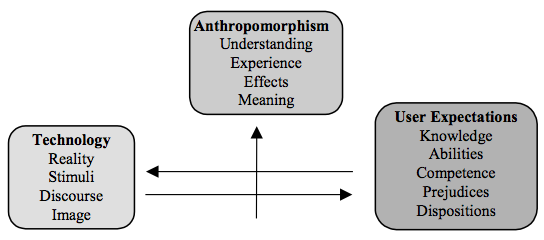
\includegraphics[scale=0.42]{persson_anthropomorphism.png}
% figure caption is below the figure
 \caption{Anthropomorphism emerges in the (real or imagined) interaction between robot and user; illustration taken from \cite{persson_anthropomorphism_2000} \hl{maybe we don't put the figure here, it was just to illustrate what I mean}}
 \label{fig:anthropomorphism_and_interaction}       % Give a unique label
 \end{figure}

We would like to take up the proposition to discriminate different levels of anthropomorphism, since each has its own characteristics and involves specific types of user expectations. This differentiation could allow to draw inferences on the human-robot relationship from the observed level of anthropomorphism.


%%%%%%%%%%%%%%%%%%%%%%%%%%%%%%%%%%%%%%%%%%%%%%%%%%%%%%%%%%%%%%%%%%%%%%%%%
%
%
%
%				DOES ANTHROPOMORPHISM MAKE ROBOTS MORE SOCIAL?
%
%
%
%%%%%%%%%%%%%%%%%%%%%%%%%%%%%%%%%%%%%%%%%%%%%%%%%%%%%%%%%%%%%%%%%%%%%%%%%


\subsection{Does anthropomorphism make robots more social?}
\label{sec:more_social}

	In general, it is suggested that increasing human-likeness of a robot	 will lead to more perceived \textit{affinity} from the human side \cite{mori_uncanny_1970}. This theoretical concept is also supported by psychological determinants of perceiving human-likeness in something non-human: \textit{"the more similar in appearance, the more people are likely to use themselves as a source of induction and anthropomorphize these nonhuman agents"} \cite{epley_seeing_2007}. Further, empirical studies have shown that robots with human-like forms can enhance social responses from humans which in turn can have a positive impact on acceptance \cite{venkatesh_theoretical_2000,duffy_anthropomorphism_2003,goetz_cooperation_2002}.  People responded more positively to an artifact that displayed human-like behavioral characteristics (emotions, facial expression) in contrast to a purely functional design \cite{eyssel_anthropomorphic_2010,krach_can_2008,reeves_media_1996,riek_how_2009}. Overall, these results suggest that human-like features in robots enhance anthropomorphism, and in turn create a social view toward the robot.

Well known from the HRI community, we may mention the other side of human-like behaviours and appearance: a not yet very well defined thin line separates acceptable human-like forms in robots from creepy artificial \textit{almost} human-like appearing robots. The underlying theory for this viewpoint is stated as the \textit{Uncanny Valley} \cite{mori_uncanny_1970} which suggests that artificial human-like forms are only acceptable up to a certain degree but lead to reluctance if they fail in trying to attain human-likeness \hl{cross-ref to later and figure}.

The theory (Figure~\ref{fig:uncanny_valley}) hypothesizes that a person's response to a human-like robot would abruptly shift from empathy to revulsion as it approached, but failed to attain, a lifelike appearance \cite{mori_uncanny_1970}. Starting with low degrees of anthropomorphic cues in a robot, humans seem to readily accept and prefer them compared to purely mechanical robots. In general, one can say that up to a certain (yet not very well defined) degree, the more human-like the robot, the more affection it can engender through familiar communication references.


\begin{figure}\centering
% Use the relevant command to insert your figure file.
% For example, with the graphicx package use
  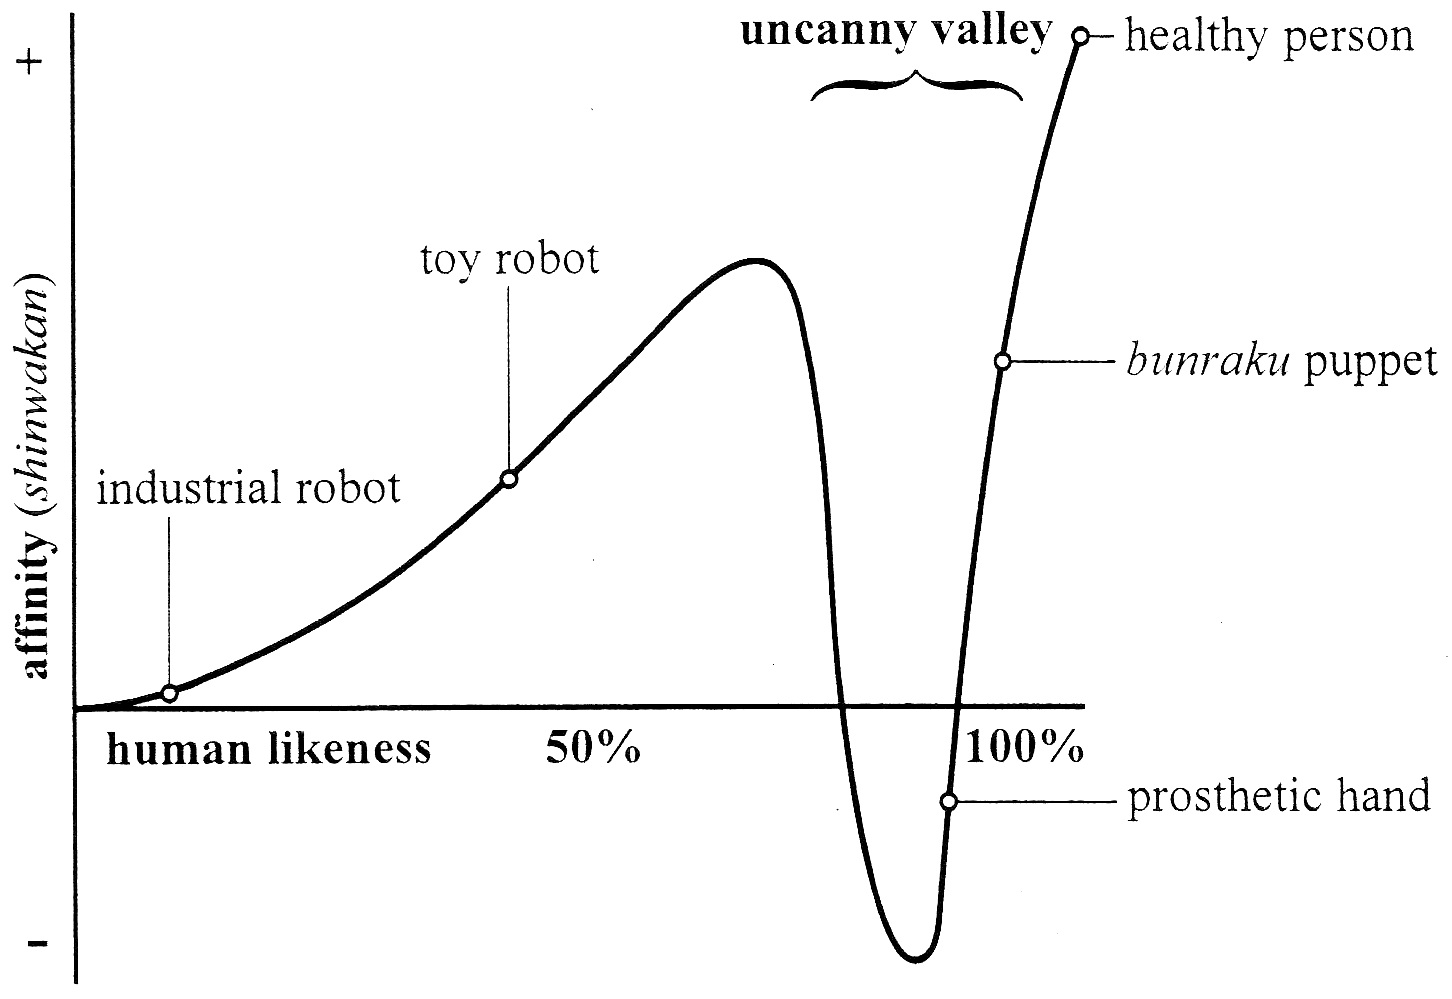
\includegraphics[scale=0.6]{uncanny-valley.jpg}
% figure caption is below the figure
 \caption{Mashiro Mori, illustration of the \textit{Uncanny Valley}, originally from 1970; picture from a manuscript version of \cite{mori_uncanny_2012}}
 \label{fig:uncanny_valley}       % Give a unique label
 \end{figure}

Another sensitive aspect is that with robots that closely resemble humans, ethical issues arise. For instance, we need to consider how far we actually want an \textit{artificial agent} to resemble ourselves and how far it should act `artificially socially' toward humans, and what happens as soon as it is considered a \textit{moral agent} \cite{sullins_when_2006}. Using \textit{socially interactive robots} in contexts involving elderly care or rehabilitation for disabled / handicapped persons, autistic children is also a controversially discussed topic \cite{robins_robots_2005}.

	
	when slowly increasing its human-likeness, the more affection 
	
The idea of the hypothesis follows Freud's description of the uncanny (a translation from the German word `unheimlich') \hl{ref Freud, The Uncanny}: "it derives its terror not from something externally alien or unknown but - on the contrary - from something strangely familiar which defeats our efforts to separate ourselves from it". \cite{hegel_understanding_2008}

	Also: Simulation Theory

	

	"The anthropomorphic design of human-machine interfaces is inevitable. The important criterion is to seek a balance between people's expectations and the machines capabilities." \cite{duffy_anthropomorphism_2002}

	"What is the ideal set of human features that could supplement and augment a robots  social functionality?" \cite{duffy_anthropomorphism_2002}


	Though, the 'anthropomorphic design principle" seems beneficial, it also raises ethical issues and has been reviewed critically in terms of acceptance. How far do we want a robot to resemble a human or act like a human?

	Findings that support anthropomorphic form in robots because they found people respond with anthropomorphizing these kind of robots, and in turn act more social toward them or accept them more easily:

	\hl{empathy --> check Iolanda's paper}

	
	
%%%%%%%%%%%%%%%%%%%%%%%%%%%%%%%%%%%%%%%%%%%%%%%%%%%%%%%%%%%%%%%%%%%%%%%%%
%
%
%
%				DYNAMICS OF ANTHROPOMORPHISM
%
%
%
%%%%%%%%%%%%%%%%%%%%%%%%%%%%%%%%%%%%%%%%%%%%%%%%%%%%%%%%%%%%%%%%%%%%%%%%%

\section{A Model of the Dynamics of Anthropomorphism}
\label{sec:dynamics_model}


\begin{figure*}[htb]
\centering


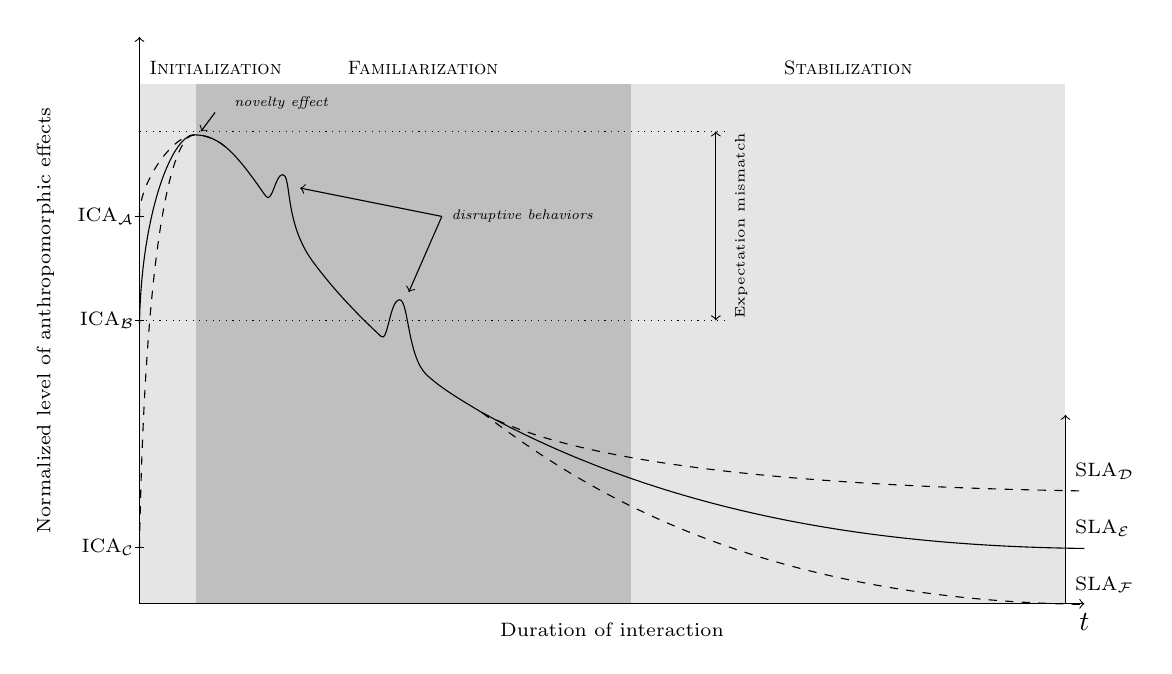
\begin{tikzpicture}[scale=1.2]

% background shading
\path[fill=gray!20] (0,0) rectangle (0.6,5.5);
\path[fill=gray!50] (0.6,0) rectangle (5.2,5.5);
\path[fill=gray!20] (5.2,0) rectangle (9.8,5.5);
\draw(0,5.5) node[anchor=south west] {\scriptsize \sc Initialization};
\draw(3,5.5) node[anchor=south] {\scriptsize \sc Familiarization};
\draw(7.5,5.5) node[anchor=south] {\scriptsize \sc Stabilization};
% horizontal axis
\draw[->] (0,0) -- (10,0) node[anchor=north] {$t$};
\draw(5,-0.1) node[anchor=north] {\scriptsize Duration of interaction};


% vertical axis
\draw[->] (0,0) -- (0,6) node[anchor=east] {};
\draw(-0.8,3) node[rotate=90,anchor=south] {\scriptsize Normalized level of anthropomorphic effects};

\draw (-0.05, 3) -- (0.05, 3) node[anchor=east] {\scriptsize $\text{ICA}_{\mathcal B}$};
\draw (-0.05, 4.1) -- (0.05, 4.1) node[anchor=east] {\scriptsize $\text{ICA}_{\mathcal A}$};
\draw (-0.05, 0.6) -- (0.05, 0.6) node[anchor=east] {\scriptsize $\text{ICA}_{\mathcal C}$};

% vertical axis - end
\draw[->] (9.8,0) -- (9.8,2) node[anchor=east] {};
\draw (9.8, 0.8) node[anchor=west] {\scriptsize SLA$_\mathcal{E}$};
\draw (9.8, 1.4) node[anchor=west] {\scriptsize SLA$_\mathcal{D}$};
\draw (9.8, .2) node[anchor=west] {\scriptsize SLA$_\mathcal{F}$};


\draw[<-] (0.65,5) -- (0.8,5.2) node[anchor=east] {};
\draw (0.9,5.3) node[anchor=west] {\tiny \it novelty effect};


\draw[dotted] (0, 5) -- (6.2,5);
\draw[dotted] (0, 3) -- (6.2,3);
\draw[<->] (6.1,3) -- (6.1,5) node[anchor=east] {};
\draw (6.2,4) node[rotate=90, anchor=north] {\tiny Expectation mismatch};

\draw[<-] (1.7,4.4) -- (3.2,4.1) node[anchor=east] {};
\draw[<-] (2.85,3.3) -- (3.2,4.1) node[anchor=east] {};
\draw (3.2,4.1) node[anchor=west] {\tiny \it disruptive behaviors};
%%%%%
%% CURVES
%%%%
\begin{scope}[yscale=-1,shift={(-0.125,-0.4)}]

% output of inkscape2tikz
\path[draw=black]
    (0.1250,-2.5620) .. controls (0.1451,-3.7193) and (0.4645,-4.5602) ..
    (0.7044,-4.5633) .. controls (0.8413,-4.5633) and (0.9599,-4.5104) ..
    (1.0794,-4.3971) .. controls (1.1989,-4.2841) and (1.3191,-4.1185) ..
    (1.4588,-3.9181) .. controls (1.5287,-3.8183) and (1.5610,-4.1413) ..
    (1.6381,-4.1420) .. controls (1.7378,-4.1420) and (1.6515,-3.6434) ..
    (1.9554,-3.2280) .. controls (2.1466,-2.9667) and (2.3889,-2.7023) ..
    (2.6819,-2.4292) .. controls (2.7551,-2.3607) and (2.7727,-2.8119) ..
    (2.8771,-2.8180) .. controls (2.9742,-2.8180) and (2.9594,-2.2108) ..
    (3.1665,-2.0209) .. controls (3.3340,-1.8673) and (3.5379,-1.7527) ..
    (3.7508,-1.6236) .. controls (5.8366,-0.4852) and (8.0977,-0.2106) ..
    (10.1250,-0.1860);
\path[draw=black, dashed]
    (0.1250,-3.6924) .. controls (0.1103,-4.0298) and (0.4645,-4.5602) .. 
    (0.7044,-4.5633)
    (3.7508,-1.6236) .. controls (4.9579,-0.9555) and (8.1358,-0.8261) .. 
    (10.1250,-0.7946);
\path[draw=black,dashed]
    (0.1250,-0.1953) .. controls (0.1804,-3.3871) and (0.4645,-4.5602) .. 
    (0.7044,-4.5633) .. controls (0.8413,-4.5633) and (0.9599,-4.5104) .. 
    (1.0794,-4.3971)
    (3.7508,-1.6236) .. controls (4.7654,-0.8505) and (6.5955,0.3538) .. 
    (10.1250,0.4062);

\end{scope}

\end{tikzpicture}

\caption{Dynamics of anthropomorphism. We distinguish three main phases:
\emph{initialization}, \emph{familiarization} and \emph{stabilization},
preceded by a \emph{pre-interaction} phase. In the pre-interaction phase,
users build an \emph{initial capital of anthropomorphism} (ICA). Once the
interaction starts, the level of anthropomorphism increases due to the
\emph{novelty effect}, and then decreases to reach a \emph{stabilized level
of anthropomorphism} (SLA).  During the interaction, unpredicted behaviors
of the robot (\emph{disruptive behaviors}) may lead to local increase of the
level of anthropomorphism.}

\label{fig:dynamics}
\end{figure*}



\subsection{Why is anthropomorphism likely to change over time?}
\label{sec:whychanges}

Why do we think that anthropomorphic projections are likely to change over time and with growing experience a person has with a robot? The underlying process in anthropomorphism is understood as reasoning about and perceiving something non-human, and unknown or unfamiliar based on one's representation of the familiar and well-known concept of being human (or one-self). The basic operations underlying inductive inference are the acquisition of knowledge, the activation or elicitation of knowledge, and the application of activated knowledge at the time of the judgment \cite{epley_when_2008}. According to Epley \textit{et al.}, the application includes attempts to correct, adjust, or integrate less accessible information into a more automatically activated default representation. This process can be seen as a process of correction, and thus, it is often insufficient leaving final judgments biased in the direction of the initially activated representation. As a person's knowledge base changes / evolves constantly with newly acquired things, or growing experiences with a robot, etc., it is likely that the "need to anthropomorphize" a robot decreases over time. First, because of the evolved knowledge about it, and second because one has familiarized oneself with it. Consequently, the robot should become more predictable and more familiar to the human user and inferences about it can be made based on the acquired knowledge.
/fxfatal{confusing paragraph...needs reformulation. Could also be turned into a section introduction instead of a subsection}


\subsection{Model of anthropomorphism over time}
\label{sec:modelintro}

So far, the HRI community has not much investigated how anthropomorphism in
human-robot interactions evolves over time (during the process of
\emph{adopting} a robot, for instance): we propose to go beyond the traditional
perception of anthropomorphism in robotics as a static feature that once
observed during a short-term interaction reflects a sustaining social effect.
Based on an extensive literature review previously published~\cite{fink_anthropomorphism_2012} and \hl{our own work} \fxfatal{Summarize
these findings in a specific section!}, we believe that anthropomorphic effects in HRI are not always the same but evolve over time, along with growing interaction
and experience with the robot, similar to how relationships among people evolve over time \hl{(cite Hinde, 1988)}. In fact, Kanda \textit{et al.} \cite{kanda_interactive_2004} also hypothesized that people's attitude toward technological artifacts and their relationship with them would evolve over time, and they were among the first who described \textit{novelty effects} during a long-term study with an interactive robot in a school.

The model of anthropomorphism we propose (Figure~\ref{fig:dynamics}) represents
how the level of anthropomorphic effects (\ie observable manifestations of
anthropomorphism, as defined in section~\ref{sec:intro}) evolves over a
long-term human-robot interaction. By long-term interaction, we mean direct
(non-mediated), repeated interaction with the same robot, over at least several
days. The nature of the interaction (goal-directed, entertainment, etc.) may
however vary.

Anthropomorphism is quantified by a \emph{normalized level of anthropomorphic
effects}: because anthropomorphic effects are not quantified on an absolute
scale, we present them as a normalized value, that spans from a minimum (no
anthropomorphic effects) to a maximum (corresponding to the novelty effect peak
on Figure~\ref{fig:dynamics}). The actual maximum value of anthropomorphic
effects depends on each unique combinations of human, robot and several other
factors we introduce below, and thus varies. The general \emph{shape} of the
model remains however the same and depicts the level of anthropomorphism over
time, \ie the general dynamics of anthropomorphism.

The model takes into account the duration of the interaction, the nature of the
interaction, as well as acquired experience and familiarization mechanisms. We
also formally introduce a so-called \emph{novelty effect} that
models the first phase of human-robot interaction, during which a specific
increase of anthropomorphic interactions is observed.

\subsection{Three phases}
\label{sec:phases}

We distinguish three main phases that describe the evolution of the
anthropomorphic effects in a long-term human-robot interaction. They are
depicted in different shades on Figure~\ref{fig:dynamics}.

First, the \emph{initialization} phase. During this short phase (from a couple
of seconds to a couple of hours), we observe an increased level of
anthropomorphism, from an \emph{initial capital of anthropomorphism}
(detailed in the next section) to a peak of anthropomorphic manifestations
that corresponds to the maximum of the \emph{novelty effect}.
Section~\ref{sec:initialization} details this first phase.

The second phase, \emph{familiarization}, lasts longer (up to several days) and
models the process of the human getting acquainted to the robot: by observation
and interaction, the human builds a model of the robot's behavior that allows
him/her to predict the robot's actions. We observe a decrease of
anthropomorphic effects during this phase, that we explain by the acquired
ability to predict the behavior of the robot: the initial apparent behavioral
complexity vanishes, and the robot is considered more and more as a tool.
Section~\ref{sec:familiarization} discusses the second phase.

The last phase is the \emph{stabilization} phase. The level of anthropomorphic
effects tends to stabilize over a longer time, to reach a \emph{stabilized
level of anthropomorphism} (SLA). The SLA may be null (no anthropomorphic
effects observed anymore), but it may also remain at a higher level.  This
third phase, as well as the \emph{stabilized level of anthropomorphism}, are
discussed in section~\ref{sec:stabilization} below.


\subsection{Initial Capital of Anthropomorphism}
\label{sec:ica}

A robot has an initial potential of being anthropomorphized. It has been shown that some \textit{people} anthropomorphism more than others, some \textit{situations} induce anthropomorphism more than others, that \textit{children} tend to anthropomorphize more than adults, and some \textit{cultures} are notorious for their anthropomorphic religions and worldviews \cite{epley_when_2008}. Our model of anthropomorphism takes these determinants into account and initializes the level of anthropomorphic interactions between a human and a robot to a value that we call \textit{initial capital of anthropomorphism} (ICA on Figure~\ref{fig:dynamics}). The ICA describes the first (real or imagined) contact to a robot. Time point $t_{0}$ can be temporally before the first real physical interaction with the robot, for instance, when a person learns about the existence of vacuum-cleaning robots and imagines using one (\eg when one watches an advertisement of the robot, or observes one at a trade show). In this stage of "pre-interaction", people form initial expectations toward the robot and imagine how they will use / interact with it. Time point $t_{0}$ can be understood as duration of interaction = 0 and user experience = 0. We build the ICA on three main factors that \textit{a priori} determine the potential that a robot will be anthropomorphized:
	
\begin{enumerate}

    \item \emph{Human-centered factor}: The \textbf{personality} and individual traits of the human user: Psychological characteristics / determinants that influence a person's tendency to anthropomorphize artifacts~\cite{epley_seeing_2007}. Other individual traits and demographic aspects are comprised (\textit{e.g.} age, gender, cultural background, professional background).
	
    \item \emph{Robot-centered factor}: The robot's \textbf{design} and how it appears to the human user. Characteristics of the robot's form, behavior, and interaction modalities (anthropomorphic design)~\cite{fong_survey_2003}.
	
    \item \emph{Situation-centered factor}: The real or imagined \textbf{purpose} of the robot, including the situational context in which it is used. The task context and role in which the robot is used / experienced (environmental context)~\cite{joosse_what_2013}.

\end{enumerate}	

The ICA comprises some hypothetical values for each of these three factors, such that different ICA values can be obtained, given the robot, human user, and environmental context\fxfatal{??}.
	
	For \textbf{personality}, we suggest to apply Epley \textit{et al.}'s \cite{epley_seeing_2007} psychological \textit{"Three Factor Theory"} of anthropomorphism. For instance, children generally tend to anthropomorphize objects more than adults. Also, a person who lacks social connection is said to be more likely to anthropomorphize. Both aspects would increase the ICA. This means that, one and the same robot used by a different user, can lead to a different ICA.
	
    For \textbf{design}, we understand that a robot that follows an anthropomorphic design (\eg NAO) leads to a higher ICA than a rather functional robot (\eg Roomba). Also, a robot that is able to display facial expressions would increase the ICA. However, \hl{as discussed before} a classification of the "amount" of anthropomorphic design in a robot, as for instance suggested by Fong \textit{et al.} \cite{fong_survey_2003}, can be difficult. Nevertheless, the important aspect is how the robot appears to the user, \eg human-like or machine-like. Studies have shown that an anthropomorphic robot is perceived differently to a non-anthropomorphic robot\fxfatal{...this sentence sounds strange like that. Need references or better integration in the paragraph}.
	
    By \textbf{purpose} we suggest that the real or imagined context in which a robot is used and the interaction that it brings along, impacts how far the robot will be attributed human-like characteristics. We	draw on findings such as presented in Joosse \textit{et al.}\fxfatal{reference?}. The authors showed that when the same robot (NAO) is used in a different task context (cleaning task \textit{vs.} tour guide), this influences the perception of the "personality" of the robot. In general, we think that a robot which is imagined to be used in a social, entertaining or playful context leads to a higher ICA than a robot which is used for a serious task (security, rescue, etc.). This idea receives support from \hl{XX (Kiesler / Goetz?)} work that revealed that people prefer a serious robot for serious tasks and a less serious robot for more playful tasks \hl{REF}. Also, we suggest that the environmental context in which people experience and interact with the robot impacts the ICA. When several people who might be friends interact simultaneously with the robot this might lead to an increased ICA \hl{study: people are more emotional when watching TV in company than when watching TV on their own}.

\subsection{Anthropomorphism during Initialization Phase}
\label{sec:initialization}

\paragraph{The Novelty Effect}
\label{sec:noveltyeffect}

\subsection{Anthropomorphism during Familiarization Phase}
\label{sec:familiarization}

\paragraph{Disruptive behaviors}
\ref{sec:disruptive}

\paragraph{Expectation mismatch}

\subsection{Anthropomorphism during Stabilization Phase}
\label{sec:stabilization}

\paragraph{Stabilized Level of Anthropomorphism (SLA)}

\fxnote{Note that ICA and SLA are NOT correlated}

%%%%%%%%%%%%%%%%%%%%%%%%%%%%%%%%%%%%%%%%%%%%%%%%%%%%%%%%%%%%%%%%%%%%%%%%%
%
%
%
%				DISCUSSION
%
%
%
%%%%%%%%%%%%%%%%%%%%%%%%%%%%%%%%%%%%%%%%%%%%%%%%%%%%%%%%%%%%%%%%%%%%%%%%%

\section{Discussion}
\label{sec:discussion}

The model of anthropomorphism we propose is still a work in progress. In
particular, its implications regarding the design of (social) robots and
human-robot interaction are still to be refined.

In this section, we discuss more speculative aspects and hypotheses that follow
from the model. These aspects would benefit further investigations and
experimental support.

\subsection{Anthropomorphism and Cognitive Models}
\label{sec:cognitivemodel}

\begin{figure}[htb]
\centering
%\resizebox{\linewidth}{!}{
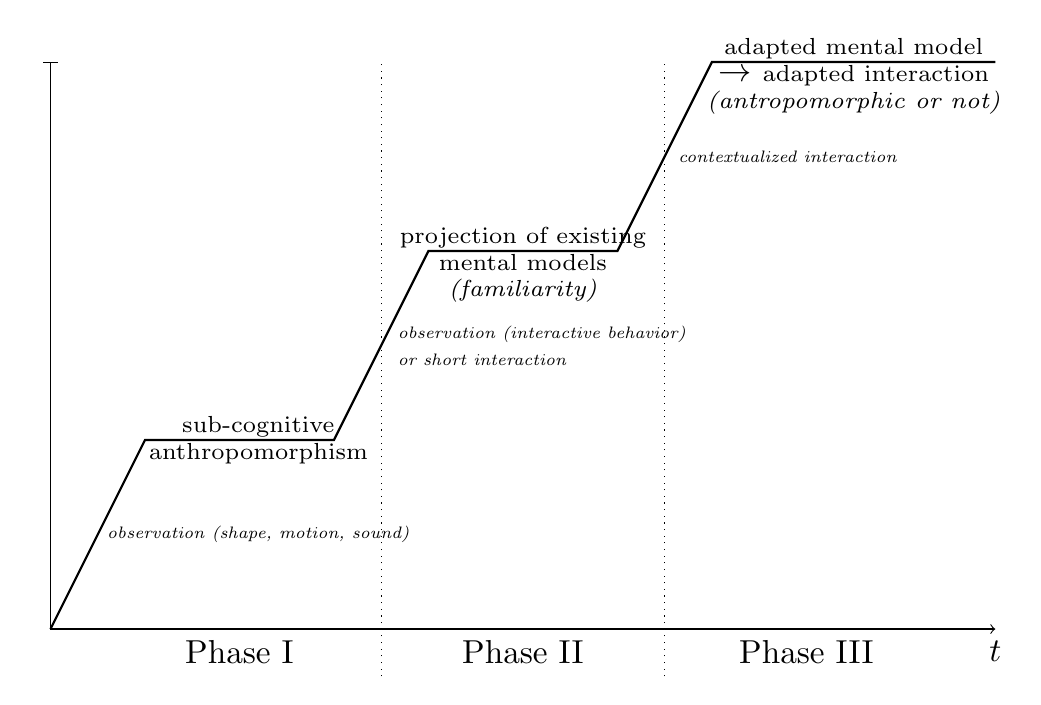
\begin{tikzpicture}[scale=1.2, transform shape]
\baselineskip=8pt

% horizontal axis
\draw[->] (0,0) -- (10,0) node[anchor=north] {$t$};
% labels
\draw   (2,0) node[anchor=north] {Phase I}
        (5,0) node[anchor=north] {Phase II}
        (8,0) node[anchor=north] {Phase III};

\draw[dotted] (3.5, -0.5) -- (3.5,6);
\draw[dotted] (6.5, -0.5) -- (6.5,6);

% vertical axis
\draw[-|] (0,0) -- (0,6) node[anchor=east] {};
% Us
\draw[thick] (0,0) -- (1,2) -- (3,2) -- (4,4) -- (6,4) -- (7,6) -- (10,6);

\draw (2.2,2) node[align=center] {\scriptsize{sub-cognitive}\\\scriptsize{anthropomorphism}}; %label
\draw (5,3.85) node[align=center] {\scriptsize{projection of existing}\\\scriptsize{mental models}\\\scriptsize{\it (familiarity)}}; %label
\draw (8.5,5.85) node[align=center] {\scriptsize{adapted mental model} \\ $\to$ \scriptsize{adapted interaction}\\\scriptsize{\it (antropomorphic or not)}}; %label

\draw (2.2,1) node[align=left] {\tiny{\it observation (shape, motion, sound)}}; %label
\draw (5.2,3) node[align=left] {\tiny \it observation (interactive behavior) \\ \tiny \it or short interaction}; %label
\draw (7.8,5) node[align=left] {\tiny \it contextualized interaction}; %label

\end{tikzpicture}
%}
\caption{The three cognitive phases of anthropomorphism: Phase I is the instinctive,
sub-cognitive identification of living peers. {\it Empathy} [TO DISCUSS] is characteristic
of this stage. After longer observation or short, uncontextualized interaction
(typically, a lab environment), the user enters Phase II: the user projects a
mental model he/she is already familiar with onto the robot. This leads to
expectation regarding the cognitive abilities of the robot. After longer {\it
contextualized} interaction (typically, at home), the user enters Phase III of
anthropomorphism: the user recomposes an accurate mental model of the robot,
based on experience. This leads to adapted interaction modalities, that may
still be anthropomorphic, or not.}
\label{fig:cognitivemodel}
\end{figure}

Figure~\ref{fig:cognitivemodel} offers a cognitive perspective on the dynamics
of anthropomorphism presented in the previous section.

The first cognitive phase we identify that contribute to anthropomorphism is
actually \emph{pre-cognitive}. Rosenthal-von der Pütten \textit{et al.} \cite{rosenthal-vonderputten_experimental_2013} investigated the neural correlates of emotional
reactions of human towards robot or other human that showed comparable
responses. \fxfatal{Complete that. Reference to the pleo paper}

After a longer observation period (typically including complete action
sequences of the robot) or short interaction (touching, short talk like
greetings), we suggest the human enters the cognitive \emph{phase II}: in this
phase, the human starts to build a behavioral and cognitive model of the robot
that would support both the observed and imagined capabilities of the robot.
The \emph{familiarity thesis}\fxfatal{citation!} would support the idea that
the human first projects onto the robot mental models of similar agents he/she
is already familiar with. This may range from animals to human adults, through
pets and children. We hypothesize that the nature of the projected mental
model, as well as how deep the human engages in this projection, might be
driven by the same parameters as we presented for the \emph{initial capital of
anthropomorphism} (section~\ref{sec:ica}).

We identify a further transition to the cognitive \emph{phase III} after a
\emph{contextualized} interaction. A \emph{contextualized} interaction is
\emph{explicitly purposeful} (the purpose of the interaction, be it purely
entertainment, is explicit and conscious for the human), and takes place in an
environment that fosters a stronger cognitive (and possibly affective)
commitment from the human in the interaction (typically, at home). During this
interaction, the human iteratively restate and reshape its behavioral and
mental model of the robot (\emph{How does the robot react to such and such
situation/input? What does the robot know about me? About itself? About our
environment? What can the robot learn?}, etc.).

This mental process heavily depends on the human understanding of the robot's
inner working, as well as his/her own tendency to anthropomorphize (the
\emph{personality} in ICA factor), but at this stage, the \emph{perception} of
the robot (its shape for instance) and its intended \emph{purpose} play a less
important role. It is mostly a human-centric process.

The result of this third phase is an iteratively adapted cognitive model of the
robot.

\paragraph{Relation to the model of anthropomorphism} It must be noted that the
three cognitive phases we introduce here do not match the
\emph{initialization}, \emph{familiarization} and \emph{stabilization} phases
introduced at~\ref{sec:phases}: in particular, cognitive phases I and II are
both included in the \emph{initialization} phase of the anthropomorphism model.

Sub-cognitive anthropomorphism typically \emph{initiates} the novelty effect by
rapidly engaging the human in the interaction through an initial projected
\emph{agency}, whereas cognitive phase II (projection of familiar mental
models) supports the novelty effect by inducing beliefs that the robot is set
up with possibly complex cognitive abilities.

The cognitive phase II also overlaps with the \emph{familiarization} phase: as
(s)he get used to the robot, we hypothesize the human restates and adapts its
cognitive model of the robot by iteratively reshaping pre-existent, familiar
models until it provides a satisfying support to explain and justify the
observed robot behavior.

A \emph{stable level of anthropomorphism} is reached when the adaptation
process depicted in cognitive phase III reached a stable state, \ie the human
experience with the robot is correctly supported by the cognitive model the
human has built.

\paragraph{Limits} This discussion on the cognitive correlates of the dynamics
of anthropomorphism are speculative, and only indirectly supported by
experimental evidence. New experiences need to be designed to specifically test
these hypothesis.\fxnote{...}

\subsection{Effect of Context of Use and Purpose of the Robot}
\label{sec:8.1}
Frederic: role of uselessness


\begin{description}
	\item[\textbf{Hypothesis 1}] A person's tendency to anthropomorphize a robot is impacted by the context of use and purpose of the robot. A social context and purpose of the robot increases anthropomorphism. \textit{(context and purpose of the robot)}
\end{description}



\subsection{Effect of Time and Familiarization}
\label{sec:8.2}

	The \textit{context of use} is related to the purpose (and functionality) of the robot and influences the user interaction experience. With \textit{time}, we refer to long-term interaction with the robot, which is related to what has been described as \textit{novelty effect} but also accounts for the user getting used to the robot. Consequently, we propose that anthropomorphism is not static but likely to change, due to what we call \textit{dynamics}, in space and time.


	As outlined in section \hl{XX}, the tendency to anthropomorphize is motivated by a person's wish to make sense of an agent which might be difficult to understand (in its functionality or behavior, for instance). In turn, a user might ascribe intentions or emotions to the system because the systems output was unexpected for the user. Based on this explanation, we estimate that when the user has familiarized herself / himself with the system, thus reached the point of when the system is usable and explainable, the tendency to anthropomorphize decreases. Therefore, our second hypothesis is as follows: 

\begin{description}
	\item[\textbf{Hypothesis 2}] A person's tendency to anthropomorphize a robot decreases over time and with growing experience the person has with the robot. \textit{(familiarize oneself with the robot)}
\end{description}	
	

Given our first hypothesis from above, this might not hold over all contexts; more concretely, probably not in a social context of usage.


	Smart innovative devices, such as personal domestic robots, might demand from a human user spontaneous usage of an unfamiliar system. Such situations will require that a user should be able to build up a mental model quickly, which particularly holds for novice users \cite{schmitz_concepts_2011}.

	Eddy \textit{et al.} points out that familiarity increases the tendency to anthropomorphize \cite{eddy_attribution_1993}.

	"As shown in several psychological experiments [13,24] and pointed out by Watt [25], familiarity may also ease social acceptance and even tend to increase people's tendency to anthropomorphize [16]." \cite{duffy_anthropomorphism_2003}

\subsection{Personal characteristic effects in anthropomorphizing}
\label{sec:8.3}

\subsection{Role of disruptive behaviors}
\label{sec:disruptive}

Common observation of naive people (children or adults) interacting with robots
shows that unexpected behaviors of the robot can have a notable impact on
interaction. \hl{cite literature, e.g. cheating robot, disagreeing, disobeying, HRI2013 paper}

During a normal interaction with the robot, the user iteratively refines his/her own
model of the behavior of the robot. As explained in previous sections, as the
user improves his/her model of the robot's actions, he/she also improves the ability to predict
the actions and thus, the user tends to anthropomorphize less.

We emit the hypothesis that an unexpected robot behavior might lead the user to
suddenly restate his/her behavioral model of the robot and will temporarily lead to
an increase of the level of anthropomorphism (depicted by the spikes on
Figure~\ref{fig:dynamics}).



\begin{figure}\footnotesize
    \begin{tabular}{  >{\centering\arraybackslash}m{2cm} | >{\centering\arraybackslash}m{2cm} | >{\centering\arraybackslash}m{2cm} }
     & Unplanned by the robot & Planned by the robot \\ \hline
    Perceived as non-intentional & case I  & case IIIa  \\ \hline
    Perceived as intentional &  case IIIb & case II 
    \end{tabular}
\caption{
    Behaviors of the robot that are unexpected by the user may be intentional
    (the robot has planned the behavior) or not (typically, a failure:
    misdetection, bug,...). Independently of that, the behavior may be
    \emph{perceived} by the user as intentional or not.}
\label{fig:perceptionUnexpectedBehavior}
\end{figure}

When talking about \emph{unexpected robot behaviors}, several distinct cases
must however be considered, summarized in Table~\ref{fig:perceptionUnexpectedBehavior}.

If the unexpected behavior is not planned, and perceived as such by the human
(case I), the human can interpret that the robot is able to fail. If the robot
explicitly states its failure (for instance, by saying ``I'm lost!''), the
behavior is then called \emph{transparent} \fixme{cite here, Julia?} \hl{(literature on transparency)}, and the
user may besides hypothesize that the robot has \emph{introspective}
capabilities \hl{(what is this?)}, which in turn may leads to higher anthropomorphism level.  On the
contrary, if the robot shows no sign of recognizing its own failure, the user
may ascribe a lower level of anthropomorphism to the robot.

In case II, the robot voluntary executes a behavior that is unexpected by the
human, and the human perceives it rightfully as an \emph{intentional} behavior.
For instance, the human asks the robot to go somewhere, and the robot refuses,
saying ``I do not want to go there''. In that case, we expect to see an
increase of anthropomorphism attribution due to the human ascribing
intentionality to the robot.

Case IIIa and IIIb correspond to misinterpretations of the robot behavior. Case
IIIb may actually lead to an increased level of anthropomorphism since the human
will (wrongfully) attribute intentionality to the robot, while case IIIa is
expected to lead to a lower anthropomorphism level.  However, in those two
cases, the next occurrence of an expected behavior, if correctly interpreted
(case I or II), is likely to lead to stronger effects due to a larger delta
between expectations and actual observed behavior. \hl{(we actually assume that anthropomorphism can be radically changing and be a very spontaneous "reaction".)}

%% experience -> unexpected behavior should not impact the interaction child-robot BEFORE the theory of mind is established!



%%%%%%%%%%%%%%%%%%%%%%%%%%%%%%%%%%%%%%%%%%%%%%%%%%%%%%%%%%%%%%%%%%%%%%%%%
%
%
%
%				CONCLUSION
%
%
%
%%%%%%%%%%%%%%%%%%%%%%%%%%%%%%%%%%%%%%%%%%%%%%%%%%%%%%%%%%%%%%%%%%%%%%%%%


\section{Conclusion}
\label{sec:9}


	Anthropomorphism is a social phenomenon, which seems to be natural on one side and very complex on the other side. It is a mechanism within oneself that makes a human observer think and treat a non-human agent as if it would have some human (social) characteristics, and ascribe to it intentions, emotions, or thoughts, for instance. In accordance with other researchers, we also think that the term is sometimes misused or misunderstood \cite{duffy_anthropomorphism_2002}. Concerning robotics, we do not think that we can speak of anthropomorphism when a person simply refers to physical parts of a robot using terms that describe a human body, such as arm, head, fingers, etc.. We believe that this is not anthropomorphism in its true sense because the person might simply take advantage of the physically resembling shape instead of truly ascribing human (social) characteristics to the robot.



\section*{Acknowledgements}
AJung Moon, Aude Billard.\\

This research was supported by the Swiss National Science Foundation through
the National Centre of Competence in Research Robotics.

\section{Bibliography}
\bibliography{dynamics-anthropomorphism}   % name your BibTeX data base

\hrule

\vspace*{.1in}
Authors' names and contact information: Julia Fink {\tt julia.fink@epfl.ch}, Séverin Lemaignan {\tt severin.lemaignan@epfl.ch}, Pierre Dillenbourg {\tt pierre.dillenbourg@epfl.ch}, CHILI Lab, EPFL, Lausanne, Switzerland.
\end{document}
